\documentclass[usenames,dvipsnames,10pt]{beamer}
\usepackage[absolute,overlay]{textpos}

% Setup appearance:
\usetheme{Boadilla}
\usefonttheme[onlylarge]{structurebold}
\usecolortheme{seahorse}
\setbeamerfont*{frametitle}{size=\normalsize,series=\bfseries}
\setbeamertemplate{navigation symbols}{}
%\setbeamercolor{frametitle}{fg=Blue}
\renewcommand\alert[1]{{\color{Magenta} #1}}
\newcommand\program[1]{\texttt{#1}}

% Packages
\usepackage[english,ukrainian]{babel}
\usepackage{times}
\usepackage[T1]{fontenc}
\usepackage{color}
\usepackage{bm}
\usepackage{slashed}
\usepackage{booktabs}% http://ctan.org/pkg/booktabs
\usepackage{xspace}
\usepackage{multirow}
\usepackage{graphicx}
\newcommand{\tabitem}{~~\llap{\textbullet}~~}
\usepackage{minted}
\usepackage{scalerel}
\usepackage{amsmath}

\hypersetup{
	colorlinks=true,
	linktoc=page,
	citecolor=Blue,
	linkcolor=Blue,
	urlcolor=Blue 
}

\setlength{\fboxsep}{0pt}%
\setlength{\fboxrule}{1pt}%

%\definecolor{stcoupcolor}{RGB}{255,0,51}

% Setup TikZ
\usepackage{tikz}
\usetikzlibrary{arrows,shapes,backgrounds,positioning}
\tikzstyle{block}=[draw opacity=0.7,line width=1.4cm]

% arrows
\tikzset{
    myarrow/.style={
        draw,
        fill=orange,
        single arrow,
        rounded corners=1,
        %        width=2ex,
        minimum width=2ex,
        minimum height=3ex,
        single arrow head extend=1ex
    }
}
\newcommand{\arrowup}{\tikz [baseline=-0.5ex]{\node [myarrow,rotate=90] {};}}
\newcommand{\arrowdown}{\tikz [baseline=-0.5ex]{\node [myarrow,rotate=-90] {};}}
\newcommand{\arrowright}{\tikz [baseline=-0.5ex]{\node [myarrow,rotate=0] {};}}
\newcommand{\arrowleft}{\tikz [baseline=-0.5ex]{\node [myarrow,rotate=180] {};}}

% draw connection
\newcommand{\tikzmark}[1]{\tikz[remember picture] \node[coordinate] (#1) {#1};}

% page numbering (backup)
\newcommand{\backupbegin}{\newcounter{finalframe}\setcounter{finalframe}{\value{framenumber}}}
\newcommand{\backupend}{\setcounter{framenumber}{\value{finalframe}}}

% Author, Title, etc.
\title[Розгортання (unfolding)]{\large Розгортання (unfolding)}
\author[Олександр Зенаєв]{Олександр Зенаєв}
\date{}

% block with custom width
\newenvironment<>{varblock}[2][.9\textwidth]{%
    \setlength{\textwidth}{#1}
    \begin{actionenv}#3%
        \def\insertblocktitle{#2}%
        \par%
        \usebeamertemplate{block begin}}
    {\par%
        \usebeamertemplate{block end}%
\end{actionenv}}

\setbeamertemplate{itemize/enumerate body begin}{\footnotesize}
\setbeamertemplate{itemize/enumerate subbody begin}{\footnotesize}

\tikzset{
    every overlay node/.style={
        rounded corners,anchor=north west,
    },
}
\def\tikzoverlay{%
    \tikz[baseline,overlay]\node[every overlay node]
}%

% main part
\begin{document}
    \begin{frame}[plain]
    %\centering\includegraphics[width=0.15\textwidth]{pics/logo/cms.png}
    %\hspace{0.1\textwidth}
    %\centering\includegraphics[width=0.18\textwidth]{pics/logo/h1}
    %\hspace{0.1\textwidth}
    %\centering\includegraphics[width=0.15\textwidth]{pics/logo/desyNEW}
    %\hspace{0.1\textwidth}
    %\centering\includegraphics[width=0.15\textwidth]{pics/logo/zeus}
    %\hspace{0.1\textwidth}
    %\centering\includegraphics[width=0.15\textwidth]{pics/logo/xFitterLogo1.png}
    
    \vspace{-0.05\textheight}
    \titlepage
    
    %\vspace{-0.15\textheight}
    %\centering\includegraphics[width=0.4\textwidth]{pics/titlepic.jpg}

    %\vspace{-0.15\textheight}
    %{\color{blue} Overview:}
    
    \vspace{0.04\textheight}
    \centering
    %place \\
    %date
\end{frame}

% number of slides w/out backup
\renewcommand{\inserttotalframenumber}{2}
\setbeamercolor{footline}{fg=blue}
\setbeamerfont{footline}{series=\bfseries}


\begin{frame}
\frametitle{Розгортання (unfolding): формулювання}
\begin{columns}
	\column{0.8\textwidth}

\vspace{-0.05\textheight}
\begin{itemize}
	\item Unfolding (розгортання, відновлення, деконволюція) в експериментальній фізиці -- математичний метод відновлення справжнього (істинного, true) розподілу фізичної величини на основі спостережуваних (виміряних, reconstructed, reco) даних
	\item Unfolding є ключовою проблемою при вимірюванні розподілів (наприклад, диференційних перерізів народження частинок, $\frac{\textrm{d}\sigma}{\textrm{d}X}$), що зазнають суттєвого впливу через обмежену роздільну здатність детектора
	\item Експериментально вимірюють диференційні перерізи, що усереднені за бінами
	\begin{eqnarray*}
		\frac{\textrm{d}\sigma}{\textrm{d}X} \sim \frac{\Delta\sigma}{\Delta X} \sim \frac{\Delta N}{\Delta X}
	\end{eqnarray*}
	\item Через обмежену роздільну здатність, події мігрують між бінами: події у справжньому біні $\Delta X_1$ можуть бути реконструйовані в іншому біні $\Delta X_2$
\end{itemize}
\column{0.2\textwidth}
	\centering{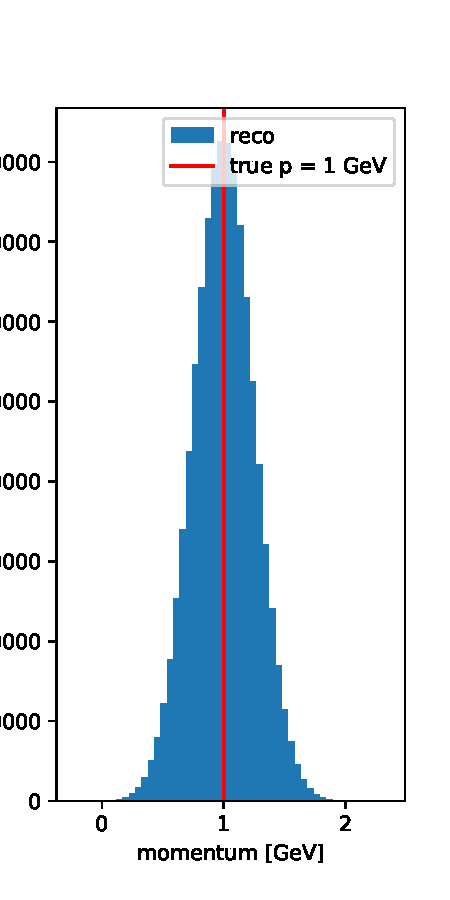
\includegraphics[width=1.2\textwidth,trim= 20 0 0 0,clip=true]{pics/smeared.pdf}}
\end{columns}

\vspace{-0.055\textheight}
\centering{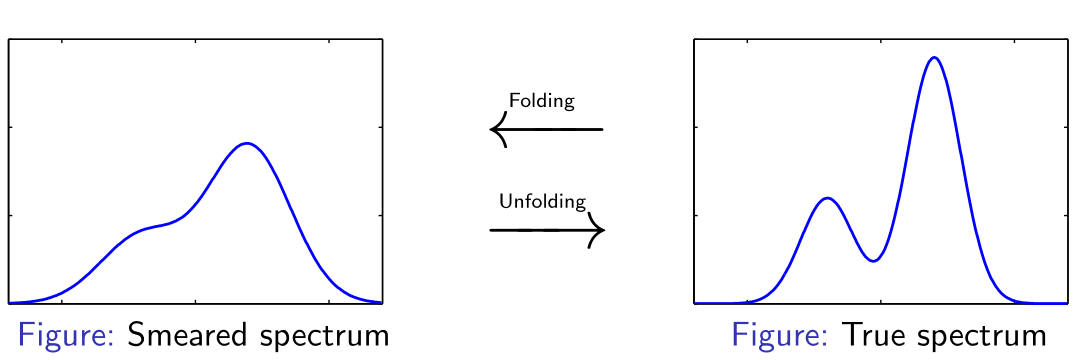
\includegraphics[width=0.61\textwidth]{pics/scr-smearing.png}\put(-200,64){\scriptsize\color{gray}M.\ Kuusela, PHYSTAT Conference on Unfolding, 2024}}
\end{frame}

\begin{frame}[fragile]
	\frametitle{Розгортання (unfolding): розв'язок}
	\begin{itemize}
		\item Задача не має однозначного розв'язку (некоректна постановка задачі, ill-posed problem): нескінчена кількість параметрів
		\item Необхідна регуляризація: 
		\begin{itemize}
			\item обмеження кількості невідомих параметрів (біни), але через статистичні похибки все одне виникають швидко осцилюючі компоненти (high frequency components)
			\item додавання додаткових обмежень на розв'язок (гладкість) для придушення швидко осцилюючих компонент
		\end{itemize}
		\item Існує декілька бібліотек для розгортання, доступних через інтерфейс \href{https://gitlab.cern.ch/RooUnfold/RooUnfold}{RooUnfold}. Інструкція: \url{https://gitlab.cern.ch/RooUnfold/RooUnfold/-/blob/master/README.md}
	\begin{minted}{bash}
	git clone https://gitlab.cern.ch/RooUnfold/RooUnfold.git
	cd RooUnfold
	mkdir build
	cd build
	cmake ..
	make -j4
	cd ..
	source build/setup.sh
	\end{minted}
		\item Ми розглянемо метод матричного розгортання, реалізований в \href{https://www.desy.de/~sschmitt/tunfold.html}{TUnfold}. Він дозволяє використовувати більшу кількість бінів на спостережуваному рівні, ніж на істинному рівні, що допомагає стабілізувати розв'язок.
	\end{itemize}
\end{frame}

\begin{frame}
	\frametitle{TUnfold (опис зі статті \href{https://www.desy.de/~sschmitt/TUnfold/tunfold\_1205.6201v5.pdf}{JINST 7 (2012) T10003 [arXiv:1205.6201] })}
	\centering{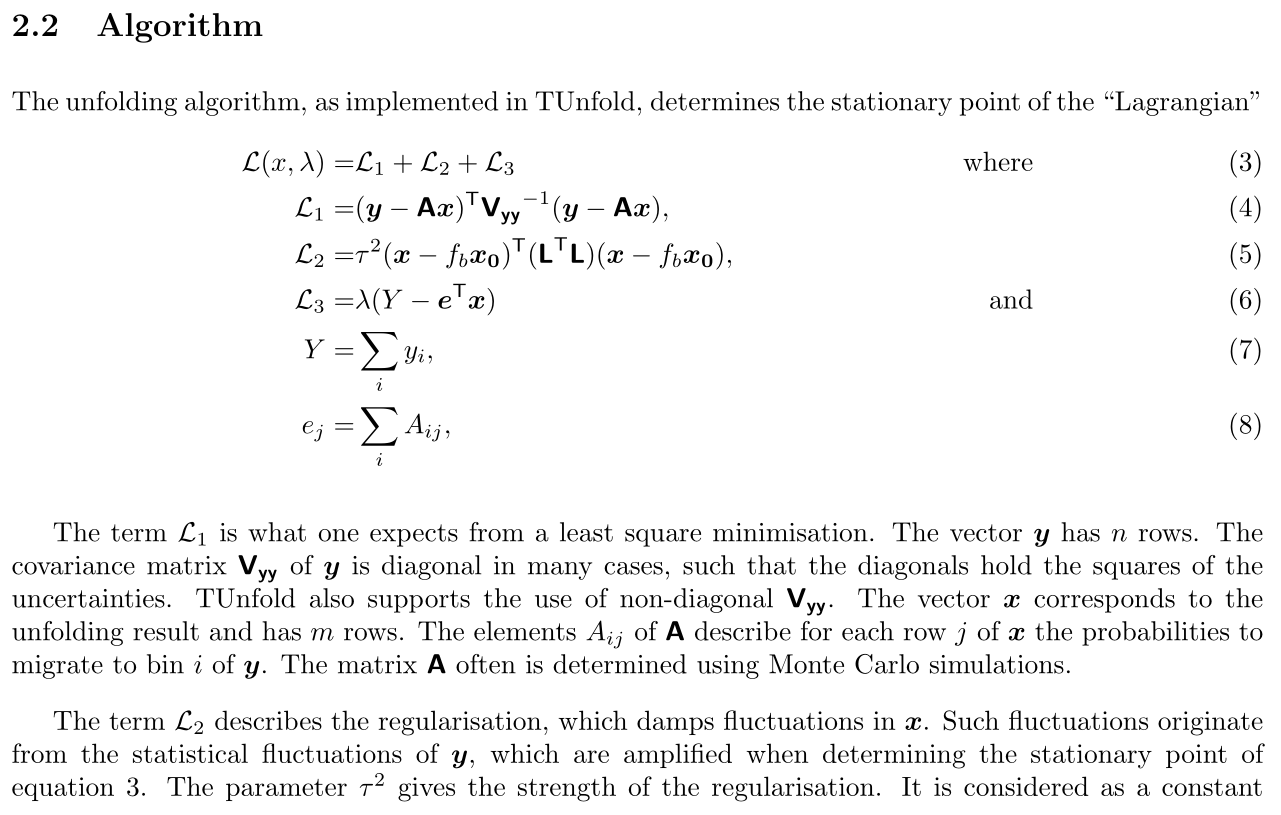
\includegraphics[width=0.9\textwidth]{pics/scr-alg.png}}
	\centering{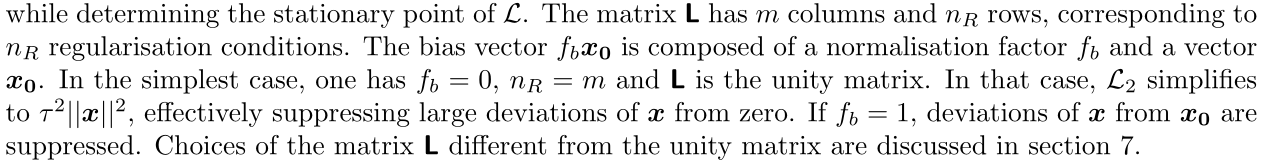
\includegraphics[width=0.9\textwidth]{pics/scr-alg2.png}}
\end{frame}

\begin{frame}
	\frametitle{Регуляризація}
	\begin{itemize}
		\item Регуляризація призначена для зменшення похибок на розв'язок (variance) ціною зміщення (викривлення) результату (bias)
		\item Ключовою проблемою є знаходження балансу між похибками і зміщенням (bias-variance tradeoff). Це можна розуміти як баланс між статистичною і систематичною похибкою.
		\item Необхідною умовою є виконання покриття (coverage): наскільки добре розв'язок описує істинний розподіл в межах похибок
		\item Концепція покриття перевіряється через тести покриття (closure tests, cover tests): використовуючи МК симуляцію (коли відомий істинний розподіл), на штучних прикладах тестують розв'язок, наскільки добре він відтворює істинний розподіл. На основі цих тестів оптимізують розгортання (обирають метод та регуляризацію)
		\item Якщо можна, краще уникати регуляризації
	\end{itemize}
\end{frame}

\begin{frame}
	\frametitle{Практичне заняття}
	\begin{itemize}
		\item Згенерувати експоненційний розподіл (імпульси частинок)
		\item Викривити згенерований розподіл, накладаючи розмиття за нормальним розподілом із додатковим зсувом
		\item Виконати розгортання за допомогою бібліотеки TUnfold (через інтерфейс RooUnfold)
		\item Порівняти результати розгортання без регуляризації та з регуляризацією
	\end{itemize}
	
	{\footnotesize 
		\vspace{0.05\textheight}
		Github:\newline \url{https://github.com/zenaiev/hep/blob/main/unfold/unfold.py}
		
		\vspace{0.05\textheight}
		Google Colab:\newline
		[under development\dots] %\scalebox{0.98}{\url{https://colab.research.google.com/github/zenaiev/hep/blob/main/unfold/unfold.ipynb}}
	}
\end{frame}

%\begin{frame}
%\frametitle{Status of xFitter releases}
%\begin{columns}\column{\dimexpr\paperwidth-10pt}
%\centering{\includegraphics[width=1.0\textwidth]{pics/pic.png}}
%\end{columns}
%\end{frame}

%\appendix
%\backupbegin
%\begin{frame}
%\frametitle{}
%\centering{\Huge \bf BACKUP}
%\end{frame}
%\backupend

\end{document}
